\newpage

\section[Day 5: Metric Spaces and Closed/Open]{ Metric Spaces \& Closed/Open }

\subsection{ Metric Spaces }

	\begin{definition}{Metric Spaces}{16cm}
		A set X is a {\color{lblue} metric space} if for any p,q $\in$ X,
		there is an associated d(p,q) $\in$ $\mathbb{R}$ such that:

		\begin{itemize}[leftmargin=1cm, itemsep=0.1cm]
			\item d(p,q) $>$ 0 \hspace{1cm} if p $\neq$ q
			
			\item d(p,q) = 0 if and only if p = q
			
			\item {\color{lgreen} Symmetry}:
				d(p,q) = d(q,p)
			
			\item {\color{lgreen} Triangle Inequality}:
				d(p,q) $\leq$ d(p,r) + d(r,q)
				\hspace{1cm}
				for any r $\in$ X.
		\end{itemize}

		For euclidean spaces $\mathbb{R}^k$,
		d(x,y) = $| x - y |$ where x,y $\in$ $\mathbb{R}^k$.
	\end{definition}

	\vspace{0.5cm}



	\begin{definition}{Types of Points and Sets}{16cm}
		For metric space X and set E $\subset$ X:
	\end{definition}
	
	\begin{enumerate}[label=(\alph*), leftmargin=2cm, itemsep=0.1cm]
		\item {\color{lblue} Neighborhood}

			\hspace{0.5cm}
			For p $\in$ X and r $>$ 0, N$_r(p)$ is the set of all q $\in$ X
			where d(q,p) $<$ r

			\begin{figure}[h]
				\centering
				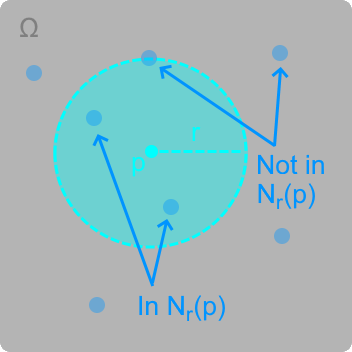
\includegraphics[scale=0.45]{Images/5.1.2a.png}
			\end{figure}

		\item {\color{lblue} Limit Points and Closed Sets}

			Closed set E contain all p $\in$ X where every N$_r(p)$ contain
			a q $\neq$ p $\in$ E

			\begin{itemize}[leftmargin=1cm, itemsep=0.1cm]
				\item Limit Points 

					\hspace{0.5cm}
					For point p $\in$ X, every N$_r(p)$ contains a
					q $\neq$ p $\in$ E

					\hspace{0.5cm}
					The set of all limit points of E = E'
				
				\item Isolated Points

					\hspace{0.5cm}
					If p $\in$ E is not a limit point of E

				\item Closed

					\hspace{0.5cm}
					If every limit point p of E is a p $\in$ E
			\end{itemize}

			\begin{figure}[h]
				\centering
				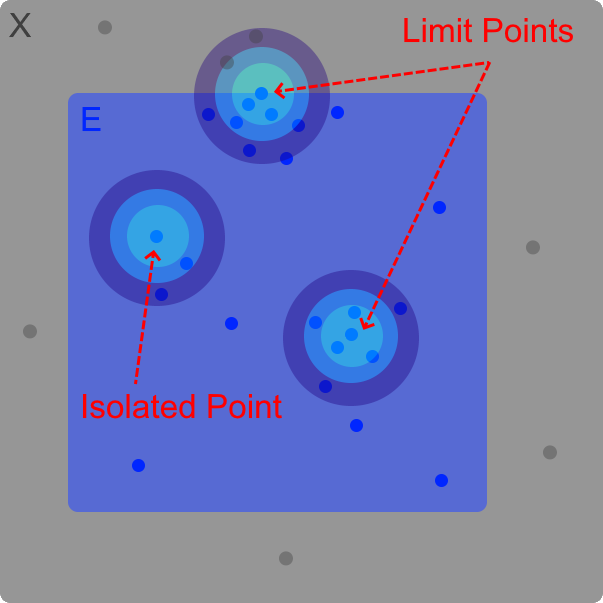
\includegraphics[scale=0.3]{Images/5.1.2b.png}
			\end{figure}

			\newpage

		\item {\color{lblue} Interior Points and Open Sets}

			Open set E contains all its p which has a N$_r(p)$ $\subset$ E
			
			\begin{itemize}[leftmargin=1cm, itemsep=0.1cm]
				\item Interior Point

					\hspace{0.5cm}
					For p $\in$ X, there is a N$_r(p)$ $\subset$ E

					\hspace{0.5cm}
					The set of all interior points = E$^o$

				\item Open

					\hspace{0.5cm}
					If every p $\in$ E is an interior point of E
			\end{itemize}

			\begin{figure}[h]
				\centering
				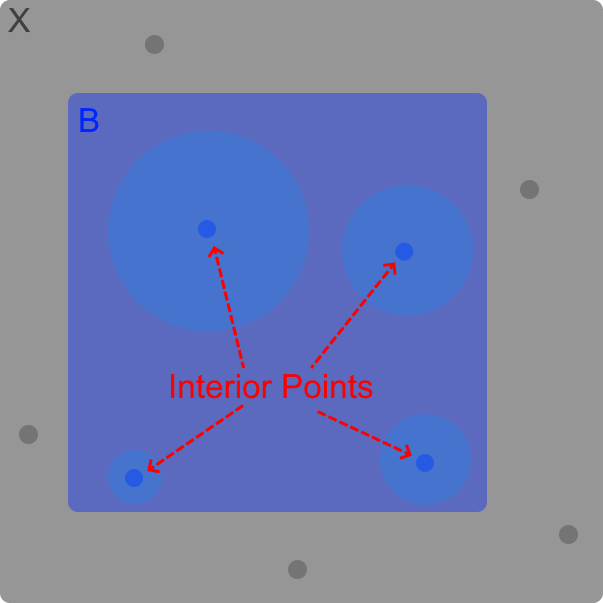
\includegraphics[scale=0.28]{Images/5.1.2c.png}
			\end{figure}

		\item {\color{lblue} More about Sets}
			
			\begin{itemize}[leftmargin=1cm, itemsep=0.1cm]
				\item Bounded

					\hspace{0.5cm}
					If there is M $\in$ $\mathbb{R}$, q $\in$ X such that
					d(p,q) $<$ M for all p $\in$ E

				\item Complement

					\hspace{0.5cm}
					From E, E$^c$ is the set of all p $\in$ X
					such that p $\not \in$ E

				\item Perfect

					\hspace{0.5cm}
					If E is closed and if every p $\in$ E is a limit point of E

				\item Dense

					\hspace{0.5cm}
					If every p $\in$ X is a limit point of E or/and p $\in$ E
					
				\item Boundary Point
				
					\hspace{0.5cm}
					For  p $\in$ X, if every N$_r(p)$ contains a
					x $\in$ E and y $\in$ E$^c$
					
					\hspace{0.5cm}
					The set of all boundary points = $\partial$E
			\end{itemize}
	\end{enumerate}

	\hspace{0.7cm}
	For a metric space X, \{X,$\emptyset$\} are both open and closed.

	\vspace{0.5cm}



	\begin{wtheorem}{N$_r(p)$ is Open}{16cm}
		Every neighborhood is an open set
	\end{wtheorem}
	
	\begin{proof}
		Let q $\in$ N$_r(p)$. Then there is a h $>$ 0 $\in$ $\mathbb{R}$
		such that d(q,p) = r - h.

		Then for any s $\in$ N$_h(q)$,
		d(s,p) $\leq$  d(s,q) + d(q,p) = h + (r - h) = r.

		Thus, for any q $\in$ N$_r(p)$, there exists a N$_h(q)$ $\subset$ N$_r(p)$.
	\end{proof}



	\begin{figure}[h]
		\centering
		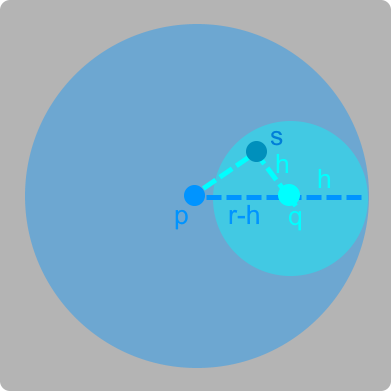
\includegraphics[scale=0.34]{Images/5.1.3.png}
	\end{figure}

	\newpage



	\begin{wtheorem}{If a set has a limit point, there are infinite q
	$\in$ E in N$_r(p)$}{16cm}
		If p is a limit point of set E, then every N$_r(p)$
		contains infinitely many q $\in$ E
	\end{wtheorem}
	
	\begin{proof}
		Suppose there is N$_{r_1}(p)$ which contains finitely many
		q = \{ q$_1$, ... , q$_n$ \}.

		Let r = min$_{m \in [1,n]}$ d(p,q$_m$). Then N$_r(p)$ contains
		no q $\in$ E such that q $\not =$ p.

		So, p is not a limit point of E which is a contradiction since
		p is a limit point of E.
	\end{proof}



	\begin{figure}[h]
		\centering
		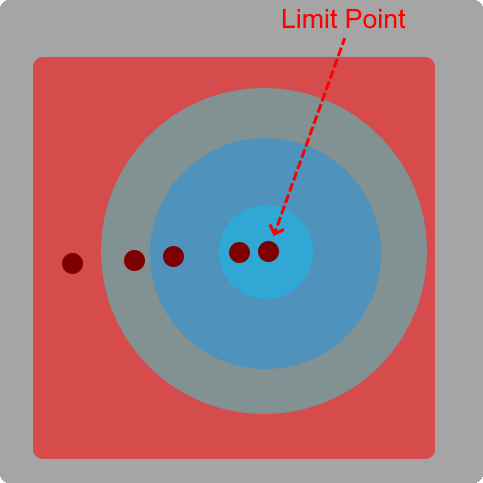
\includegraphics[scale=0.31]{Images/5.1.4.png}
	\end{figure}



	\begin{corollary}{Limit points do not exist in Finite sets}{16cm}
		A finite set E has no limit points.
		Since E' = $\emptyset$ $\in$ E, all finite set must be closed.		
	\end{corollary}
	
	\begin{proof}
		Let p be a limit point of finite set E. By {\color{red} theorem 5.1.4}, 
		then any N$_r(p)$ contain infinite q $\in$ E so E is an infinite set
		which is a contradiction since E is finite.

		So p cannot be limit point of E and thus, E has no limit points.
		Since finite set E contains all its limit points because there are no
		limit points, then E is closed.
	\end{proof}

	\vspace{0.5cm}



	\begin{wtheorem}{De Morgan's Laws}{16cm}
		Let $E_1, E_2 , ... $ be a collection of sets. Then,
		($\cup_{}^{}$ $E_x$)$^\text{c}$ = $\cap_{}^{}$ ($E_x$$^\text{c}$).		 
	\end{wtheorem}
	 
	\begin{proof}
		If p $\in$ ($\cup_{}^{}$ $E_x$)$^\text{c}$, then
		p $\not \in$ ($\cup_{}^{}$ $E_x$).

		Thus, p $\not \in$ $E_x$ for any x so p $\in$ E$_x^\text{c}$ for all x.
		Thus, p $\in$ $\cap_{}^{}$ ($E_x^c$) so
		($\cup_{}^{}$ $E_x$)$^c$ $\subset$ $\cap_{}^{}$ ($E_x^c$).

		If p $\in$ $\cap_{}^{}$ ($E_x^c$), then p $\in$ $E_x^c$ for all x.
		
		Thus, p $\not \in$ $E_x$ for any x so p $\not \in$ $\cup_{}^{}$ $E_x$.
		Thus, p $\in$ ($\cup_{}^{}$ $E_x$)$^c$ so
		$\cap_{}^{}$ ($E_x^c$) $\subset$ ($\cup_{}^{}$ $E_x$)$^c$.
		
		Thus, ($\cup_{}^{}$ $E_x$)$^c$ = $\cap_{}^{}$ ($E_x^c$). 
	\end{proof}



	\begin{figure}[h]
		\centering
		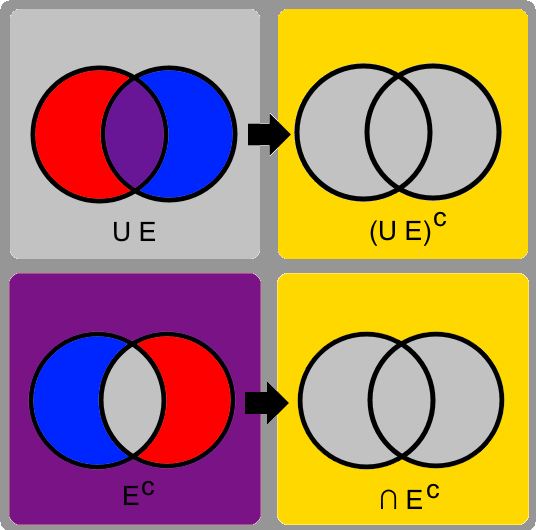
\includegraphics[scale=0.35]{Images/5.1.6.png}
	\end{figure}

	\newpage



	\begin{wtheorem}{Open set $\rightarrow$ Closed complement}{16cm}
		A set E is open if and only if E$^\text{c}$ is closed
	\end{wtheorem}
	
	\begin{proof}
		Suppose E is open. Let x be a limit point of E$^c$.

		Then for every r $>$ 0, N$_r(x)$ must contain a p $\in$ E$^c$
		such that p $\neq$ x.

		Then, N$_r(x)$ $\not \subset$ E so x is not an interior point of E and
		thus, x $\not \in$ E so x $\in$ E$^c$.

		Since any limit point x of E$^c$ is a x $\in$ E$^c$, then E$^c$ is closed.

		\vspace{0.2cm}

		Suppose E$^c$ is closed. Let x $\in$ E.

		Since x $\not \in$ E, x is not a limit point of E.
		Then there exists a r $>$ 0 such that any p $\in$ N$_r(x)$ is not in E.
		Thus, every p $\in$ N$_r(x)$ is p $\in$ E so N$_r(x)$ $\subset$ E and thus,
		x is an interior point of E.
		Since any x $\in$ E is an interior point of E, then E is open.
	\end{proof}

	\vspace{0.5cm}



	\begin{corollary}{Closed set $\rightarrow$ Open complement}{16cm}
		A set F is closed if only only if F$^\text{c}$ is open
	\end{corollary}
	
	\begin{proof}
		From {\color{red} theorem 5.1.7}, let E = F$^\text{c}$
	\end{proof}

	\vspace{0.5cm}



	\begin{ltheorem}{Union: open $\rightarrow$ open and
	Intersection: closed $\rightarrow$ closed}{1.5cm}
		\item If $\{G_x\}$ is a finite or infinite collection of open sets,
		then $\cup$ $G_x$ is open.

			\begin{proof}[15.5cm]
				If p $\in$ $\cup$ $G_x$, then p $\in$ $G_x$ for at least one x.
				Let $\overline{x}$ be such an x.

				Since $G_{\overline{x}}$ is open, then p is an interior point of
				$G_{\overline{x}}$ and thus, there is a N$_r(p)$ such that
				N$_r(p)$ $\subset$ $G_{\overline{x}}$ $\subset$ $\cup$ $G_x$.
				So p is an interior point of $\cup$ $G_x$.

				Since any p $\in$ $\cup$ $G_x$ is an interior point, then
				$\cup$ $G_x$ is open.
			\end{proof}

		\item If $\{F_x\}$ is a finite or infinite collection of closed sets,
		then $\cap$ $F_x$ is closed.

			\begin{proof}[15.5cm]
				By {\color{red} theorem 5.1.7}, any $F_x^c$ is open.
				Since $\{F_x^c\}$ is a finite or infinite collection of
				open set, then by part (a), $\cup$ $F_x^c$ is open.

				Thus, again by {\color{red} theorem 5.1.7},
				($\cup$ $F_x^c$)$^c$ is closed.

				By {\color{red} theorem 5.1.6},
				($\cup$ $F_x^c$)$^c$ = $\cap$ $(F_x^c)^c$
				= $\cap$ $F_x$.
			\end{proof}

		\item If $G_1, ... , G_n$ is a finite collection of open sets,
		then $\cap_{x=1}^n$ $G_x$ is open.

			\begin{proof}[15.5cm]
				If p $\in$ $\cap_{x=1}^n$ $G_x$, then p $\in$ $G_x$ for
				all $G_x$ for x = \{1, 2, ... , n\}.

				Since each $G_x$ is open, then for any $G_x$, there is a
				N$_{r_x}(p)$ $\subset$ $G_x$.

				Let r = min($r_1, r_2 , ... , r_n$).
				Thus, p $\in$ N$_r(p)$ $\subset$ N$_{r_x}(p)$ for all x.

				So, N$_r(p)$ $\subset$ $\cap_{x=1}^n$ $G_x$ and thus,
				p is an interior point of $\cap_{x=1}^n$ $G_x$ so
				$\cap_{x=1}^n$ $G_x$ is open.

				\vspace{0.1cm}

				{\color{purple} Infinite + Closed}: $G_i$ = $(-1/i,1/i)$
				\hfill
				{\color{purple} Infinite + Open}: $G_i$ = $(-i,i)$
			\end{proof}

		\item If $F_1, ... , F_n$ is a finite collection of closed sets,
		then $\cup_{x=1}^n$ $F_x$ is closed.

			\begin{proof}[15.5cm]
				By {\color{red} theorem 5.1.7}, any $F_x^c$ is open.
				Since $F_1^c, ... , F_n^c$ is a finite collection of
				open set, then by part (c), $\cap_{x=1}^n$ $F_x^c$ is open.

				Thus, again by {\color{red} theorem 5.1.7},
				($\cap_{x=1}^n$ $F_x^c$)$^c$ is closed.

				By {\color{red} theorem 5.1.6},
				($\cap_{x=1}^n$ $F_x^c$)$^c$ = $\cup_{x=1}^n$ $(F_x^c)^c$
				= $\cup_{x=1}^n$ $F_x$.

				\vspace{0.1cm}

				{\color{purple} Infinite + Closed}: $F_i$ = $[-1/i,1/i]$
				\hfill
				{\color{purple} Infinite + Open}: $F_i$ = $[1/i,\infty)$
			\end{proof}	 
	\end{ltheorem}

	\newpage



	\begin{wtheorem}{E' is Closed}{16cm}
		Let  E $\subset$ X. Then, (E')' $\subset$ E'.
		Thus, E' is closed.
	\end{wtheorem}
	
	\begin{proof}
		If x $\in$ (E')', then for every $N_{r_1}(x)$, there is a
		y $\not =$ x where y $\in$ E'.
		
		Since y $\in$ E', then for every $N_{r_2}(y)$
		where $r_2$ $<$ d(x,y), there is a
		z $\not =$ x,y where z $\in$ E.

		Let r = $r_1$ + $r_2$.

		Then for every N$_r(x)$, there exists a z $\not =$ x where
		z $\in$ E.
		Thus, x $\in$ E' so (E')' $\subset$ E'.
	\end{proof}

	\vspace{0.5cm}



	\begin{wtheorem}{E$^o$ is Open}{16cm}
		Let  E $\subset$ X. Then, E$^o$ is open. 
	\end{wtheorem}
	
	\begin{proof}
		If p $\in$ E$^o$, there is a r $>$ 0 such that
		N$_r(p)$ $\subset$ E.

		Then for 0 $<$ s $<$ r, N$_s(p)$ $\subset$ N$_r(p)$
		so any q $\in$ N$_s(p)$ is q $\in$ E$^o$.

		Since any p $\in$ E$^o$ have a N$_s(p)$ $\subset$ E$^o$,
		then E$^o$ is open.
	\end{proof}

	\vspace{0.5cm}





\subsection{ Intervals and Balls } 

	\begin{definition}{Segments and Intervals}{16cm}
		In $\mathbb{R}$, a {\color{lblue} segement} is an open interval
		(a,b) = \{ x $\in$ $\mathbb{R}$ : a $<$ x $<$ b \}

		In $\mathbb{R}$, a {\color{lblue} interval} is a closed interval
		[a,b] = \{ x $\in$ $\mathbb{R}$ : a $\leq$ x $\leq$ b \}
	\end{definition}

	\vspace{0.5cm}



	\begin{definition}{Open Balls}{16cm}
		In $\mathbb{R}^k$, an {\color{lblue} open ball} of radius
		r $>$ 0 centered at p is:

		\qquad N$_r(p)$ = \{ x $\in$ $\mathbb{R}^k$ : $|x-p|$ $<$ r \}
		= \{ x $\in$ $\mathbb{R}^k$ : d(x,p) $<$ r \}

		A {\color{lblue} closed ball} has d(x,p) $\leq$ r.
	\end{definition}
	
	\vspace{0.5cm}



	\begin{definition}{Convex}{16cm}
		E $\subset$ $\mathbb{R}^k$ is {\color{lblue} convex} if for all
		x,y $\in$ E and t $\in$ [0,1], tx + (1-t)y $\in$ E.
	\end{definition}
	
	\vspace{0.5cm}



	\begin{example}
		Balls in $\mathbb{R}^k$ are convex
	\end{example}

	\begin{tbox}
		Let x,y $\in$ open ball N$_r(p)$. Let z = tx + (1-t)y for t $\in$ [0,1].
		
		Since $|x - p| < r$ and $|y - p| < r$:

		\hspace{1cm}
		$|z - p|$ = $|tx + (1-t)y - p|$
		= $|tx + (1-t)y - tp + (t-1)p|$

		\hspace{2.3cm}
		= $|t(x-p) + (1-t)(y-p)|$ $\leq$ $t|(x-p)|$ + $(1-t)|(y-p)|$

		\hspace{2.3cm}
		$<$ tr + (1-t)r = r

		Thus, z $\in$ N$_r(p)$ so balls are convex.
		Same proof applies to closed balls.	
	\end{tbox}

	\vspace{0.5cm}



	\begin{definition}{Dense}{16cm}
		E $\subset$ X is {\color{lblue} dense} if every x $\in$ X is either in E or
		a limit point of E.
	\end{definition}
	
	\vspace{0.5cm}



	\begin{example}
		Let X = $\mathbb{R}$. Then, E = $\mathbb{Q}$ is dense in $\mathbb{R}$.
	\end{example}

	\begin{tbox}
		Fix x $\in$ $\mathbb{R}$ and r $>$ 0.
		There is a q $\in$ $\mathbb{Q}$ such that x-r $<$ q $<$ x.
		So for any r $>$ 0 and q $\in$ $\mathbb{Q}$, q $\neq$ x and
		q $\in$ N$_r(x)$.
		Thus, every x $\in$ $\mathbb{R}$ is a limit point of $\mathbb{Q}$.
	\end{tbox}
	 



